\chapter{Flare-Finding Algorithm}
\label{app:Flares}

\par The algorithm used to find flares is performed as such (see also Figure \ref{fig:BurstAlg}):

\begin{enumerate}
  \item Choose some threshold values $T_L$ and $T_H$.  Set the value of all datapoints below $T_L$ to zero.
  \item Retrieve the x-co-ordinate of the highest value remaining in the dataset.  Call this value $x_m$ and store it in a list.
  \item Set the value of point at $x_m$ to zero.
  \item Scan forwards from $x_m$.  If the selected point has a nonzero value, set it to zero and move to the next point.  If the selected point has a zero value, move to step (v).
  \item Scan backwards from $x_m$.  If the selected point has a nonzero value, set it to zero and move to the previous point.  If the selected point has a zero value, move to step (vi).
  \item Retrieve the y-co-ordinate of the highest value remaining in the dataset.  Call this $y_m$.
  \item If $y_m>T_H$, repeat steps (ii)--(vi).  If $y_m<T_H$, proceed to step (viii).
  \item Restore the original dataset.
  \item Retrieve the list of $x_m$ values found in step (ii).  Sort them in order of size.
  \item For each pair of adjacent $x_m$ values, find the x-coordinate of the datapoint between them with the lowest y-value.  Call these values $x_c$.
  \item This list of $x_c$ can now be used to demarcate the border between peaks.
\end{enumerate}

\begin{figure}
    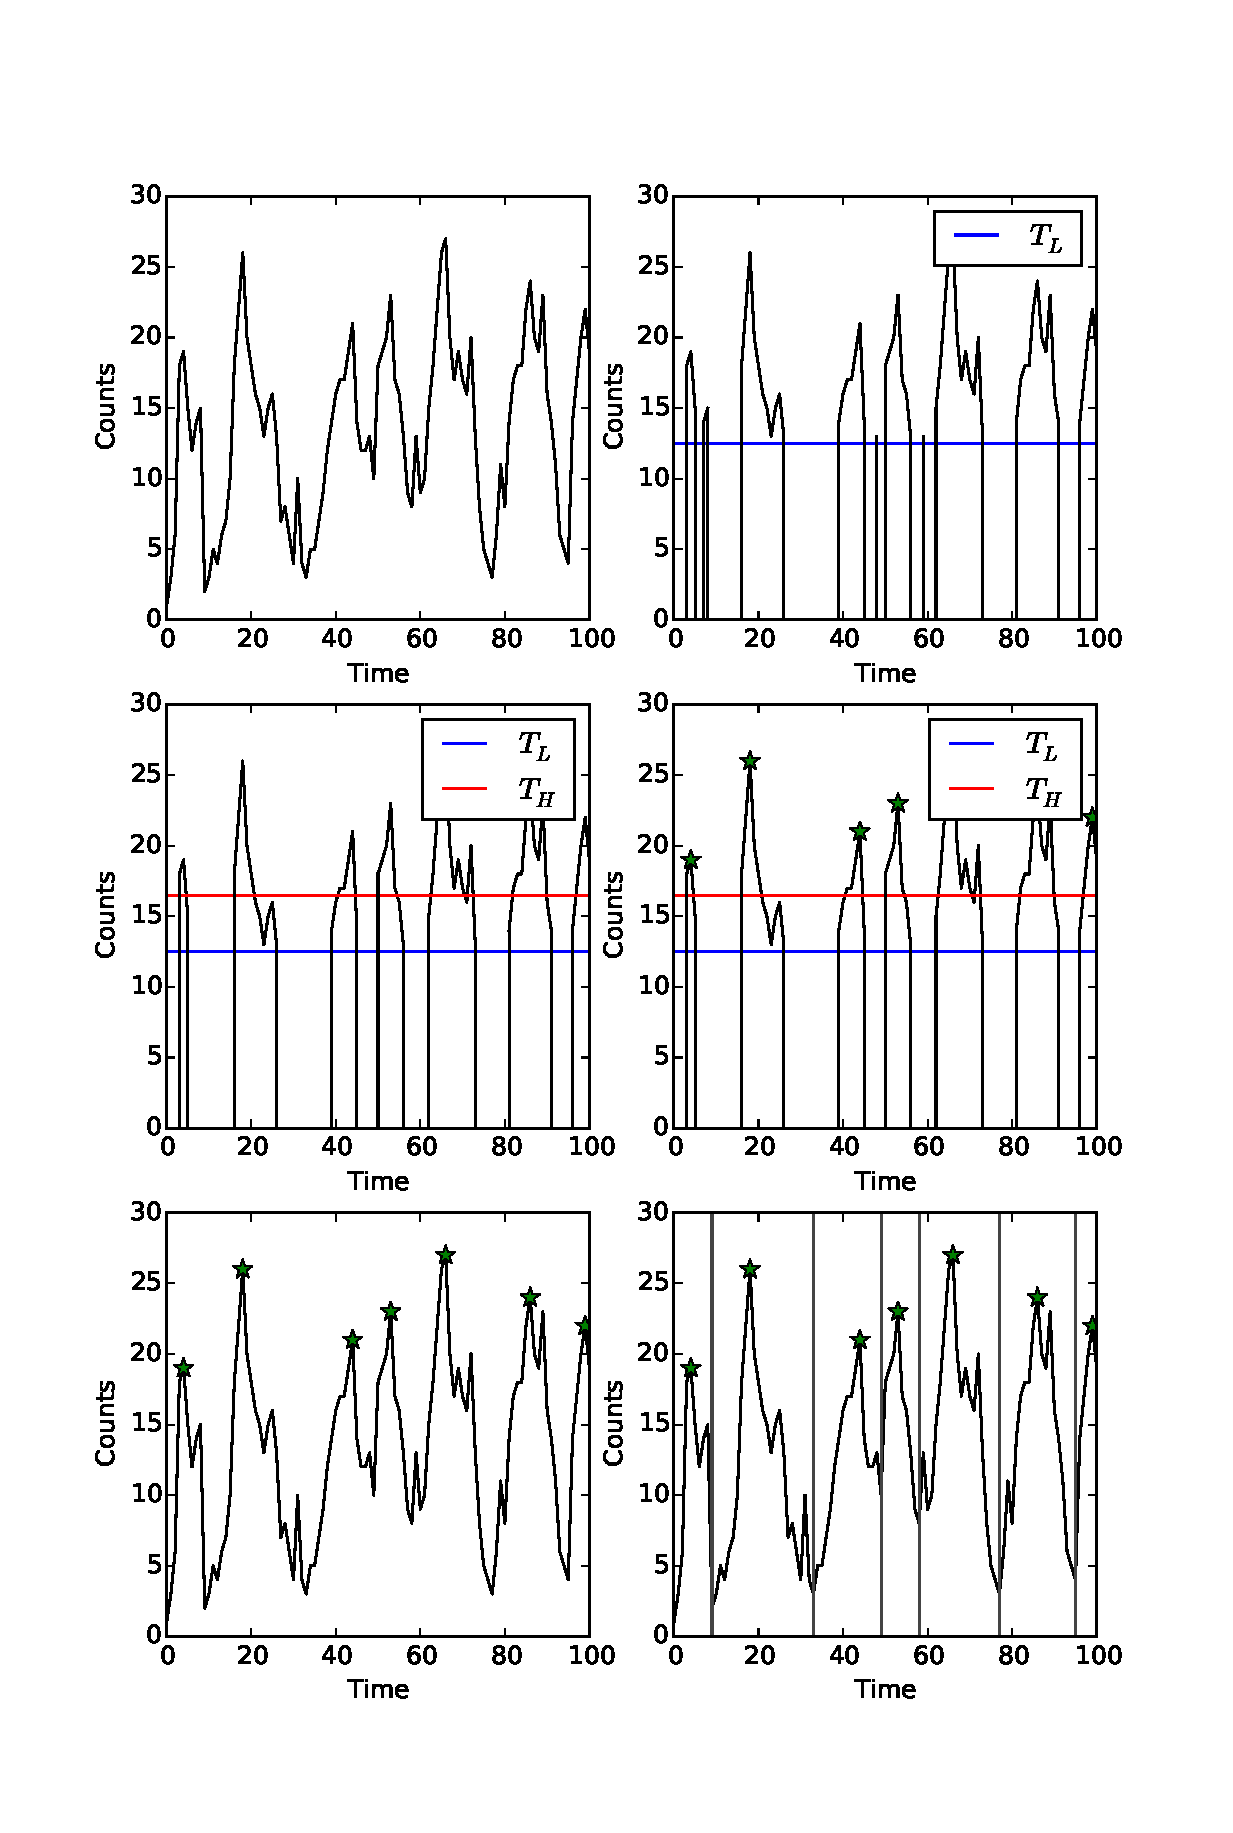
\includegraphics[width=\columnwidth, trim = 0mm 30mm 0mm 28mm]{images/steps.eps}
    \captionsetup{singlelinecheck=off}
    \caption{From top-left: (i) An untouched data-set.  (ii) The dataset with all $y<T_L$ removed.  (iii) The dataset with all contiguous nonzero regions with $\max(y)<T_H$ removed.  (iv) The peak x-values $x_m$.  (v) The restored dataset with the peak x-values $x_m$ highlighted.  (vi) The boundaries between adjacent peaks.}
   \label{fig:BurstAlg}
\end{figure}

The values $T_L$ and $T_H$ can also be procedurally generated for a given piece of data:

\begin{enumerate}
  \item Select a small section of the dataset or a similar dataset (containing $\sim20$ peaks by eye) and note the location $x_e$ of all peaks found by eye.
  \item Let $P_L$ and $P_H$ be two arbitrary values in the range $[0,100]$.
  \item Let $T_L$ ($T_H$) be the $P_L$th ($P_H$th) percentile of the y-values of the subsection of dataset.
  \item Run the flare-finding algorithm up to step (ix).  Save the list of $x_m$.
  \item Split the dataset into bins on the x-axis such as the bin width $b\ll p$, where $p$ is the rough x-axis separation between peaks.
  \item For each bin, note if you found any value in $x_m$ falls in the bin and note if any value of $x_e$ falls in the bin.
  \item Using each bin as a trial, compute the Heidke Skill Score \citep{Heidke_SKSC} of the algorithm with the method of finding peaks by eye:
  \begin{equation}HSS = \frac{2(AD-BC)}{(A+B)(B+D)+(A+C)(C+D)}
  \label{eq:HSS}
  \end{equation}
  Where $A$ is the number of bins that contain both $x_e$ and $x_m$, $B$ ($C$) is the number of bins that contain only $x_m$ ($x_e$) and $D$ is the number of bins which contain neither \citep{Kok_YesNo}.
  \item Repeat steps (iii)--(vii) for all values of $P_H>P_L$ for $P_L$ and $P_H$ in $[1,100]$.  Use a sensible value for the resolution of $P_L$ and $P_H$.  Save the HSS for each pair of values
  \item Locate the maximum value of HSS, and note the $P_L$ and $P_H$ values used to generate it.  Use these values to generate your final $T_L$ and $T_H$ values.
\end{enumerate}

We show an example of Heidke skill score grid for this algorithm, applied to a Class IV observation, in Figure \ref{fig:Heidke}.

\begin{figure}
    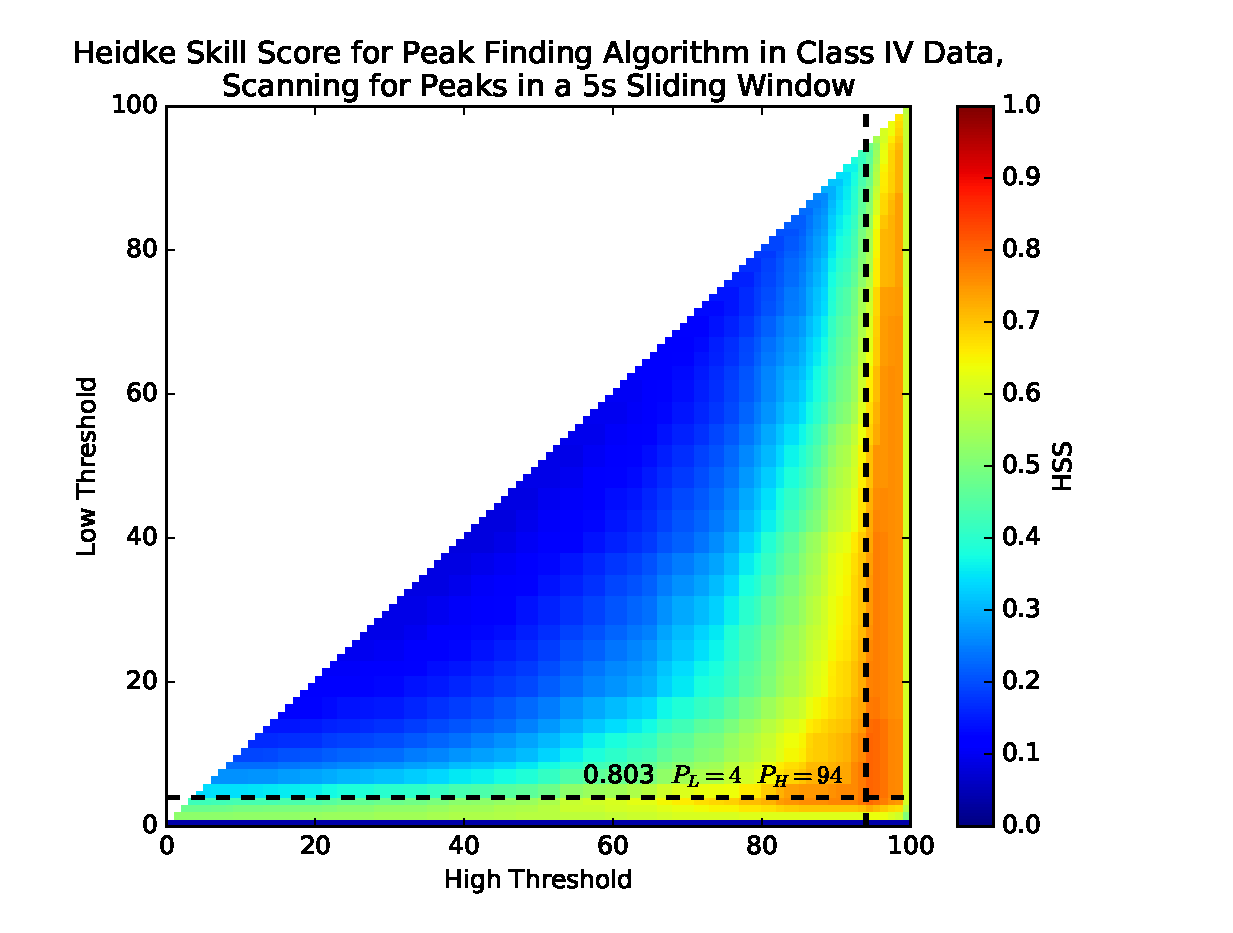
\includegraphics[width=\columnwidth, trim = 0mm 10mm 0mm 10mm]{images/HSS_J.eps}
    \captionsetup{singlelinecheck=off}
    \caption{The Heidke Skill score of a Class IV observation of IGR J17091-3624 for a selection of different values $P_L$ and $P_H$.}
   \label{fig:Heidke}
\end{figure}
